\subsection{Experiment B: Larger Network and Heterogeneous Fleet}

\label{subsec:experiment-b}

Experiment B uses six heterogeneous helicopters and seven demand areas, with 20, 30, 40, 50 and 60 tasks and 30 generated instances per size. Greedy Benefit and Greedy Density are compared with three initializations of the same MILP: cold HiGHS, a Benefit start and a Density start. All methods use the primary-output benefit in Section~3.3. Each MILP treatment receives independent solve allowances of 1, 5, 15, 60, 600 and 1800 s. The 1800-s runs provide the main comparison; Section~4.3 examines shorter budgets. Allowances are HiGHS parameters, not hard wall-clock deadlines.



At 1800 s, cold HiGHS and the Benefit and Density starts certified 116/150, 116/150 and 116/150 instances, respectively. Greedy Benefit had mean paired shortfalls of 11.9--17.4\% across task counts. Greedy Density had mean paired shortfalls of 12.8--17.7\% across task counts.

Shortfalls use the 116/150 instances with a certified reference for this model and objective. Table notes give the counts at each size. Benefit and completed-task means include all generated instances, including uncertified runs; absent plans are scored separately as idle=0.


\begin{figure}[!htbp]
\centering
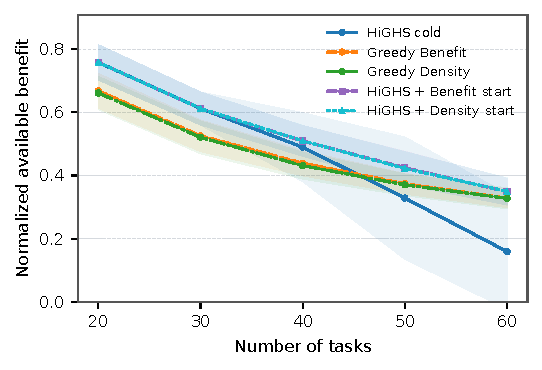
\includegraphics[width=\columnwidth]{B1_solution_quality_coverage_aware.pdf}
\caption{Experiment B benefit at the 1800-s MILP allowance. 
Lines show means over the same 30 instances at each task count; bands show
one sample standard deviation. The three MILP initialization strategies are drawn separately.}
\label{fig:expB-quality}
\end{figure}


Among matched runs in which both methods certified, median end-to-end time differences relative to cold were HiGHS + Benefit start: +0.46 s (116 pairs); HiGHS + Density start: +0.22 s (116 pairs).


\begin{figure*}[!htbp]
\centering
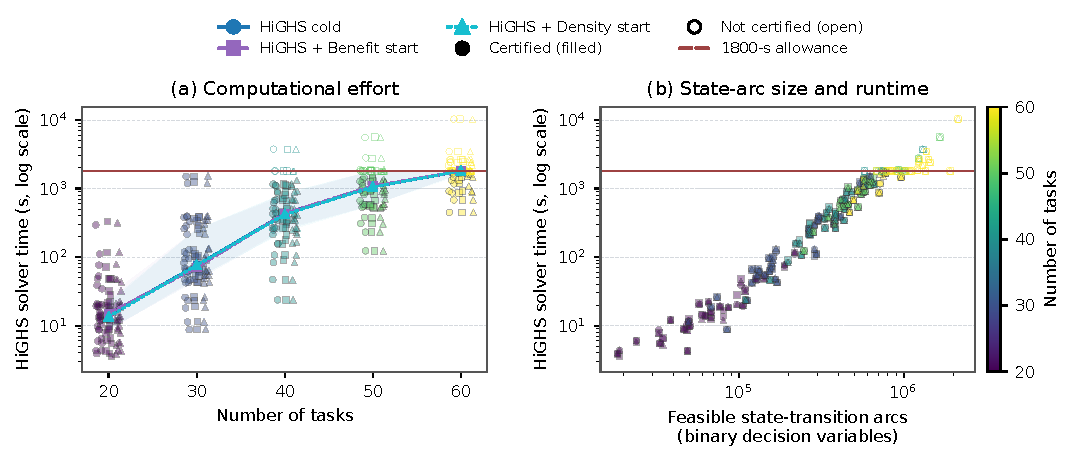
\includegraphics[width=\textwidth]{B8_computational_effort.pdf}
\caption{Experiment B computational effort. Panel (a) shows solver
times with medians and interquartile ranges; panel (b) relates solver time to
generated state-transition arcs. Marker shape identifies the initialization.
Filled markers denote certified runs; open markers, when present, denote
uncertified runs. The dashed line is the 1800-s solver allowance.
Table~\ref{tab:expB-runtime} includes preparation time.}
\label{fig:expB-effort}
\end{figure*}


\begin{table}[!htbp]
\centering
\caption{Experiment B: solution quality and certification at the 1800-s MILP budget.}
\label{tab:expB-quality}
\scriptsize
\setlength{\tabcolsep}{2.6pt}
\renewcommand{\arraystretch}{1.08}
\begin{tabular}{@{}ccccc@{}}
\toprule
Tasks & \makecell{Normalized available\\benefit\\Mean $\pm$ SD} & \makecell{Completed tasks\\Mean $\pm$ SD} & \makecell{Certified\\runs} & \makecell{Shortfall\\(\%)} \\
\midrule
\multicolumn{5}{@{}l}{\textit{Panel A: HiGHS cold}}\\
\addlinespace[0.2em]
20 & $0.7581 \pm 0.0559$ & $18.60 \pm 0.89$ & $30/30$ & 0.0 \\
30 & $0.6122 \pm 0.0523$ & $23.33 \pm 1.58$ & $30/30$ & 0.0 \\
40 & $0.4896 \pm 0.1092$ & $24.83 \pm 5.65$ & $27/30$ & 0.0 \\
50 & $0.3285 \pm 0.1936$ & $21.00 \pm 12.37$ & $20/30$ & 0.0 \\
60 & $0.1591 \pm 0.1825$ & $12.10 \pm 14.15$ & $9/30$ & 0.0 \\
\midrule
\multicolumn{5}{@{}l}{\textit{Panel B: Greedy Benefit}}\\
\addlinespace[0.2em]
20 & $0.6681 \pm 0.0549$ & $17.57 \pm 1.33$ & -- & 11.9 \\
30 & $0.5257 \pm 0.0500$ & $21.40 \pm 1.52$ & -- & 14.1 \\
40 & $0.4389 \pm 0.0401$ & $24.23 \pm 1.72$ & -- & 14.7 \\
50 & $0.3737 \pm 0.0326$ & $26.33 \pm 2.01$ & -- & 16.1 \\
60 & $0.3280 \pm 0.0297$ & $27.30 \pm 2.35$ & -- & 17.4 \\
\midrule
\multicolumn{5}{@{}l}{\textit{Panel C: Greedy Density}}\\
\addlinespace[0.2em]
20 & $0.6611 \pm 0.0523$ & $17.73 \pm 1.26$ & -- & 12.8 \\
30 & $0.5208 \pm 0.0517$ & $22.33 \pm 1.37$ & -- & 15.0 \\
40 & $0.4312 \pm 0.0427$ & $25.60 \pm 1.48$ & -- & 16.5 \\
50 & $0.3704 \pm 0.0343$ & $27.30 \pm 2.00$ & -- & 16.6 \\
60 & $0.3276 \pm 0.0331$ & $28.97 \pm 2.24$ & -- & 17.7 \\
\midrule
\multicolumn{5}{@{}l}{\textit{Panel D: HiGHS + Benefit start}}\\
\addlinespace[0.2em]
20 & $0.7581 \pm 0.0559$ & $18.60 \pm 0.89$ & $30/30$ & 0.0 \\
30 & $0.6122 \pm 0.0523$ & $23.33 \pm 1.58$ & $30/30$ & 0.0 \\
40 & $0.5093 \pm 0.0486$ & $26.00 \pm 2.29$ & $27/30$ & 0.0 \\
50 & $0.4245 \pm 0.0518$ & $27.93 \pm 2.38$ & $20/30$ & 0.0 \\
60 & $0.3486 \pm 0.0425$ & $28.23 \pm 2.98$ & $9/30$ & 0.0 \\
\midrule
\multicolumn{5}{@{}l}{\textit{Panel E: HiGHS + Density start}}\\
\addlinespace[0.2em]
20 & $0.7581 \pm 0.0559$ & $18.60 \pm 0.89$ & $30/30$ & 0.0 \\
30 & $0.6122 \pm 0.0523$ & $23.33 \pm 1.58$ & $30/30$ & 0.0 \\
40 & $0.5097 \pm 0.0486$ & $26.20 \pm 2.28$ & $27/30$ & 0.0 \\
50 & $0.4221 \pm 0.0526$ & $28.20 \pm 2.54$ & $20/30$ & 0.0 \\
60 & $0.3497 \pm 0.0426$ & $28.97 \pm 3.38$ & $9/30$ & 0.0 \\
\bottomrule
\end{tabular}
\begin{minipage}{0.98\columnwidth}
\footnotesize
Means and sample SD summarize the same instances for all five variants. All MILP variants receive 1800 s. Shortfalls are computed per instance against a certified optimum of the same model and objective, then averaged; unknown optima are excluded. Certified-reference counts: 20 tasks: 30/30; 30 tasks: 30/30; 40 tasks: 27/30; 50 tasks: 20/30; 60 tasks: 9/30. Certification denotes HiGHS optimal status at relative MIP tolerance 1e-06; it is not applicable to the greedy policies. If no incumbent is returned, a separately available idle plan contributes zero benefit and zero tasks. Raw incumbent values remain missing.
\end{minipage}
\end{table}


\begin{table}[!htbp]
\centering
\caption{Experiment B: computational performance and generated state-arc MILP size.}
\label{tab:expB-runtime}
\scriptsize
\setlength{\tabcolsep}{2.4pt}
\renewcommand{\arraystretch}{1.08}
\begin{tabular}{@{}ccccc@{}}
\toprule
Tasks & \makecell{Runtime\\Mean $\pm$ SD} & \makecell{Maximum\\runtime} & \makecell{Variables\\mean} & \makecell{Constraints\\mean} \\
\midrule
\multicolumn{5}{@{}l}{\textit{Panel A: HiGHS cold (seconds)}}\\
\addlinespace[0.2em]
20 & $31.85 \pm 55.52$ & $297.51$ & 84{,}274 & 30{,}945 \\
30 & $209.22 \pm 336.73$ & $1512.75$ & 211{,}166 & 66{,}316 \\
40 & $659.14 \pm 748.26$ & $3761.75$ & 413{,}162 & 108{,}489 \\
50 & $1286.71 \pm 1040.37$ & $5625.95$ & 655{,}107 & 147{,}902 \\
60 & $2064.36 \pm 1677.47$ & $10343.86$ & 1{,}019{,}518 & 193{,}893 \\
\midrule
\multicolumn{5}{@{}l}{\textit{Panel B: Greedy Benefit (milliseconds)}}\\
\addlinespace[0.2em]
20 & $1.262 \pm 0.925$ & $6.143$ & -- & -- \\
30 & $1.432 \pm 0.072$ & $1.615$ & -- & -- \\
40 & $1.882 \pm 0.108$ & $2.151$ & -- & -- \\
50 & $2.539 \pm 0.869$ & $5.774$ & -- & -- \\
60 & $3.756 \pm 1.719$ & $8.734$ & -- & -- \\
\midrule
\multicolumn{5}{@{}l}{\textit{Panel C: Greedy Density (milliseconds)}}\\
\addlinespace[0.2em]
20 & $0.946 \pm 0.069$ & $1.136$ & -- & -- \\
30 & $1.286 \pm 0.090$ & $1.607$ & -- & -- \\
40 & $1.711 \pm 0.135$ & $2.130$ & -- & -- \\
50 & $2.176 \pm 0.144$ & $2.495$ & -- & -- \\
60 & $2.856 \pm 1.012$ & $8.135$ & -- & -- \\
\midrule
\multicolumn{5}{@{}l}{\textit{Panel D: HiGHS + Benefit start (seconds)}}\\
\addlinespace[0.2em]
20 & $33.52 \pm 61.65$ & $333.83$ & -- & -- \\
30 & $209.60 \pm 338.78$ & $1497.82$ & -- & -- \\
40 & $665.82 \pm 742.93$ & $3747.63$ & -- & -- \\
50 & $1292.43 \pm 1039.66$ & $5635.91$ & -- & -- \\
60 & $2067.36 \pm 1674.80$ & $10332.76$ & -- & -- \\
\midrule
\multicolumn{5}{@{}l}{\textit{Panel E: HiGHS + Density start (seconds)}}\\
\addlinespace[0.2em]
20 & $32.57 \pm 59.66$ & $320.18$ & -- & -- \\
30 & $210.42 \pm 337.79$ & $1520.61$ & -- & -- \\
40 & $667.02 \pm 752.74$ & $3750.98$ & -- & -- \\
50 & $1280.87 \pm 1039.72$ & $5619.31$ & -- & -- \\
60 & $2067.23 \pm 1674.32$ & $10329.44$ & -- & -- \\
\bottomrule
\end{tabular}
\begin{minipage}{0.98\columnwidth}
\footnotesize
End-to-end time includes network and matrix generation, native conversion, model loading and solving. Warm variants additionally include greedy construction, mapping, validation and submission. Preparation is charged to each treatment although shared within the batch. Greedy runtimes are in milliseconds. The common MILP size is reported once. The solver allowance excludes preparation and is not a guaranteed end-to-end deadline.
\end{minipage}
\end{table}

